\documentclass{article}
\usepackage{v-test-paper}
\newenvironment{solution}{\par\noindent\color{red!85!black}$\Rightarrow$\vspace{0em}}{}
\title{\textsc{JEE Advanced 2010 Paper-I\\Physics}}
\date{}
\begin{document}
\maketitle
\begin{enumerate}
    
\begin{enumerate}
    \item In a historical experiment to determine Planck's constant, a metal surface was irradiated with light of different wavelengths. The emitted photoelectron energies were measured by applying a stopping potential. The relevant data for the wavelength (\(\lambda\)) of incident light and the corresponding stopping potential (\(V_0\)) are given below:
    \begin{center}
        \begin{tabular}{ccc}
        \hline
        \(\lambda (\mu m)\) & \(V_0 (Volt)\) \\
        \hline
        0.3 & 2.0 \\
        0.4 & 1.0 \\
        0.5 & 0.4 \\
        \hline
        \end{tabular}
    \end{center}
    Given that \( c = 3 \times 10^8 m\ s^{-1} \) and \( e = 1.6 \times 10^{-19} C \), Planck's constant (in units of J s) found from such an experiment is
    \begin{tasks}(2)
        \task \( 6.0 \times 10^{-34} \)
        \task \( 6.4 \times 10^{-34} \)
        \task \( 6.6 \times 10^{-34} \)
        \task \( 6.8 \times 10^{-34} \)
    \end{tasks}
\end{enumerate}

    
\item In the arrangement of Fig. 1.9 the masses \( m_0 \), \( m_1 \), and \( m_2 \) of bodies are equal, the masses of the pulley and the threads are negligible, and there is no friction in the pulley. Find the acceleration \( w \) with which the body \( m_0 \) comes down, and the tension of the thread binding together the bodies \( m_1 \) and \( m_2 \), if the coefficient of friction between these bodies and the horizontal surface is equal to \( k \). Consider possible cases.
    \begin{center}
        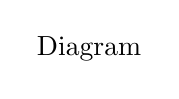
\begin{tikzpicture}
            \node at (0, 0) {Diagram};
        \end{tikzpicture}
    \end{center}

    
\begin{enumerate}
    \item A current carrying wire heats a metal rod. The wire provides a constant power (P) to the rod. The metal rod is enclosed in an insulated container. It is observed that the temperature (T) in the metal rod changes with time (t) as
    \[
    T(t) = T_0(1 + \beta t)^{\frac{1}{4}},
    \]
    where \(\beta\) is a constant with appropriate dimension while \(T_0\) is a constant with dimension of temperature. The heat capacity of the metal is;
        \begin{tasks}(2)
            \task \(\frac{4P(T(t)-T_0)^3}{\beta^4 T_0}\)
            \task \(\frac{4P(T(t)-T_0)^4}{\beta^4 T_0^5}\)
            \task \(\frac{4P(T(t)-T_0)^2}{\beta^4 T_0^3}\)
            \task \(\frac{4P(T(t)-T_0)}{\beta^4 T_0^2}\)
        \end{tasks}
\end{enumerate}

    
\item A point moves rectilinearly in one direction. Fig. 1.1 shows the distance \( s \) traversed by the point as a function of the time \( t \).
    \begin{center}
        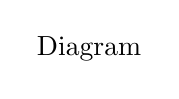
\begin{tikzpicture}
            \node at (0, 0) {Diagram}; % Replace this with the actual TikZ code for the diagram.
        \end{tikzpicture}
    \end{center}
Using the plot find:
\begin{itemize}
    \item the average velocity of the point during the time of motion;
    \item the maximum velocity;
    \item the time moment \( t_0 \) at which the instantaneous velocity is equal to the mean velocity averaged over the first \( t_0 \) seconds.
\end{itemize}

    \item A disc of mass \( m = 50 \) g slides with the zero initial velocity down an inclined plane set at an angle \( \alpha = 30^\circ \) to the horizontal; having traversed the distance \( l = 50 \) cm along the horizontal plane, the disc stops. Find the work performed by the friction forces over the whole distance, assuming the friction coefficient \( k = 0.15 \) for both inclined and horizontal planes.
    \begin{center}
        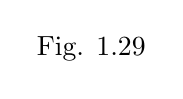
\begin{tikzpicture}
            \node at (0, 0) {Fig. 1.29};
        \end{tikzpicture}
    \end{center}\begin{solution}
    \begin{center}
        \begin{tikzpicture}
            \pic at (0, 0) {frame=3cm};
        \end{tikzpicture}
    \end{center}

    \begin{align*}
        \intertext{Let \(s\) be the distance covered by the disk along the incline, from the equation of increment of mechanical energy of the disk in the field of gravity: \(\Delta T + \Delta U - A_{fr}\)}
        0 + (-mgs\sin\alpha) &= -kmg\cos\alpha \cdot s - kmgl\\
        \intertext{or}
        s &= \dfrac{kl}{\sin\alpha - k\cos\alpha} \tag{1}
        \intertext{Hence the sought work}
        A_{fr} &= -kmg[s \cos\alpha + l]\\
        A_{fr} &= -\dfrac{klmg}{1 - k \cos\alpha} \quad \text{(using Eq. 1)}
        \intertext{On putting the values}
        A_{fr} &= -0.05 \, \text{J}
    \end{align*}
\end{solution}
    \item Two bars of masses $m_1$ and $m_2$ connected by a non-deformed light spring rest on a horizontal plane. The coefficient of friction between the bars and the surface is equal to $k$. What minimum constant force has to be applied in the horizontal direction to the bar of mass $m_1$ in order to shift the other bar?
\begin{solution}
    \begin{center}
        \begin{tikzpicture}
            \pic at (0, 0) {frame=3cm};
        \end{tikzpicture}
    \end{center}

    \begin{align*}
        \intertext{Let \(x\) be the compression in the spring when the bar \(m_2\) is about to shift. Therefore at this moment spring force on \(m_2\) is equal to the limiting friction between the bar \(m_2\) and horizontal floor. Hence}
        \kappa x &= km_2 g \quad \text{[where \(\kappa\) is the spring constant (say)]} \quad \tag{1}
        \intertext{For the block \(m_1\) from work-energy theorem:}
        A &= \Delta T = 0 \text{ for minimum force. (A here includes the work done in stretching the spring.)}
        \intertext{So,}
        Fx - \dfrac{1}{2} \kappa x^2 - km_1 g x &= 0 \quad \text{or} \quad \kappa \dfrac{x}{2} = F - km_1 g \quad \tag{2}
        \intertext{From Eqs. (1) and (2),}
        F &= kg \left(m_1 + \dfrac{m_2}{2}\right)
    \end{align*}
\end{solution}

    
\begin{enumerate}
    \item Two loudspeakers \(M\) and \(N\) are located 20 m apart and emit sound at frequencies 118 Hz and 121 Hz, respectively. A car is initially at a point \(P\), 1800 m away from the midpoint \(Q\) of the line \(MN\) and moves towards \(Q\) constantly at 60 km/hr along the perpendicular bisector of \(MN\). It crosses \(Q\) and eventually reaches a point \(R\), 1800 m away from \(Q\). Let \(v_P\), \(v_Q\) and \(v_R\) be the beat frequencies measured by a person sitting in the car at time \(t\). Let \(v(t)\) represent the beat frequency measured by a person sitting in the car at time \(t\). The speed of sound in air is 330 m s\(^{-1}\). Which of the following statement(s) is(are) true regarding the sound heard by the person?
        \begin{tasks}(1)
            \task \(v_P + v_R = 2 v_Q\)
            \task The rate of change in beat frequency is maximum when the car passes through \(Q\)
            \task The plot below represents schematically the variation of beat frequency with time (with a labeled diagram indicating points \(P\), \(Q\), and \(R\).)
            \task The plot below represents schematically the variation of beat frequency with time (with a labeled diagram indicating points \(P\), \(Q\), and \(R\).)
        \end{tasks}
\end{enumerate}
\begin{center}
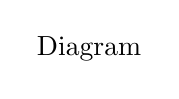
\begin{tikzpicture}
\node {Diagram};
\end{tikzpicture}
\end{center}

    
\item A spherical metal shell A of radius $R_A$ and a solid metal sphere B of radius $R_B$ ($R_B < R_A$) are kept far apart and each is given charge $`+Q'$. Now they are connected by a thin metal wire. Then
    \begin{tasks}(2)
        \task $E_{\text{inside}}^A = 0$
        \task $Q_A > Q_B$
        \task $\frac{\sigma_A}{\sigma_B} = \frac{R_B}{R_A}$
        \task $E_{\text{on surface}}^A < E_{\text{on surface}}^B$
    \end{tasks}

    
\begin{enumerate}
\item A ball is thrown from ground at an angle $\theta$ with horizontal and with an initial speed $u_0$. For the resulting projectile motion, the magnitude of average velocity of the ball up to the point when it hits the ground for the first time is $V_1$. After hitting the ground, the ball rebounds at the same angle $\theta$ but with a reduced speed of $u_0/\alpha$. Its motion continues for a long time as shown in figure. If the magnitude of average velocity of the ball for entire duration of motion is $0.8 V_1$, the value of $\alpha$ is \_\_\_\_\_\_\_.

\begin{center}
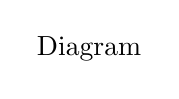
\begin{tikzpicture}
\node {Diagram};
\end{tikzpicture}
\end{center}

\end{enumerate}

    
\item A series R-C circuit is connected to AC voltage source. Consider two cases; (A) when C is without a dielectric medium and (B) when C is filled with dielectric of constant 4. The current $I_R$ through the resistor and voltage $V_C$ across the capacitor are compared in the two cases. Which of the following is/are true?
    \begin{tasks}(2)
        \task $I^A_R > I^B_R$
        \task $I^A_R < I^B_R$
        \task $V^A_C > V^B_C$
        \task $V^A_C < V^B_C$
    \end{tasks}

    
\item A cubical region of side \( a \) has its centre at the origin. It encloses three fixed point charges, \( -q \) at \( (0, -a/4, 0) \), \( +3q \) at \( (0,0,0) \) and \( -q \) at \( (0,+a/4,0) \). Choose the correct option(s).
    \begin{center}
        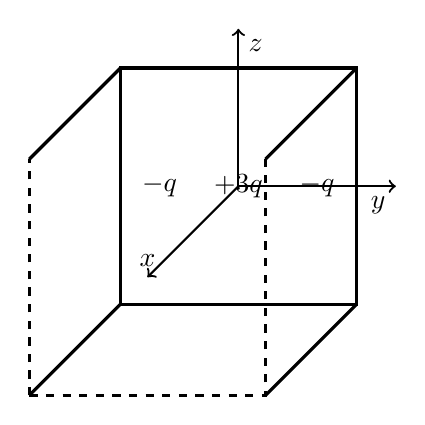
\begin{tikzpicture}
            % Drawing the cube with charges, as a simple representation
            \draw[very thick] (-1.5,-1.5,0) -- (-1.5,1.5,0) -- (1.5,1.5,0) -- (1.5,-1.5,0) -- cycle; % base
            \draw[very thick] (-1.5,-1.5,0) -- (-1.5,-1.5,3);
            \draw[very thick] (-1.5,1.5,0) -- (-1.5,1.5,3);
            \draw[very thick] (1.5,1.5,0) -- (1.5,1.5,3);
            \draw[very thick] (1.5,-1.5,0) -- (1.5,-1.5,3);

            \draw[very thick, dashed] (-1.5,-1.5,3) -- (1.5,-1.5,3) -- (1.5,1.5,3); % top
            \draw[very thick, dashed] (-1.5,-1.5,3) -- (-1.5,1.5,3);

            % Charges
            \node at (-1, 0, 0) { \( -q \) };
            \node at (0, 0, 0) { \( +3q \) };
            \node at (1, 0, 0) { \( -q \) };

            % Axes
            \draw[thick,->] (0,0,0) -- (2,0,0) node[anchor=north east] {\( y \)};
            \draw[thick,->] (0,0,0) -- (0,2,0) node[anchor=north west] {\( z \)};
            \draw[thick,->] (0,0,0) -- (0,0,3) node[anchor=south] {\( x \)};
        \end{tikzpicture}
    \end{center}
    \begin{tasks}(2)
        \task The net electric flux crossing the plane \( x = +a/2 \) is equal to the net electric flux crossing the plane \( x = -a/2 \).
        \task The net electric flux crossing the plane \( y = +a/2 \) is more than the net electric flux crossing the plane \( y = -a/2 \).
        \task The net electric flux crossing the entire region is \( \frac{q}{\varepsilon_0} \).
        \task The net electric flux crossing the plane \( z = +a/2 \) is equal to the net electric flux crossing the plane \( x = +a/2 \).
    \end{tasks}

    \item A horizontal plane with the coefficient of friction \( k \) supports two bodies: a bar and an electric motor with a battery on a block. A thread attached to the bar is wound on the shaft of the electric motor. The distance between the bar and the electric motor is equal to \( l \). When the motor is switched on, the bar, whose mass is twice as great as that of the other body, starts moving with a constant acceleration \( w \). How soon will the bodies collide?\begin{solution}
    \begin{center}
        \begin{tikzpicture}
            \pic at (0, 0) {frame=3cm};
        \end{tikzpicture}
    \end{center}
    
    \begin{align*}
        \intertext{From the Newton’s second law in projection form}
        \text{For the bar,} \quad T - 2 \ k \ m \ g &= (2m) \ w \tag{1}\\
        \text{For the motor,} \quad T - kmg &= mw' \tag{2}\\
        \intertext{Now, from the equation of kinematics in the frame of bar or motor}
        l &= \frac{1}{2} (w + w') \ t^2 \tag{3}\\
        \intertext{From Eqs. (1), (2) and (3) we get on eliminating $T$ and $w'$}
        t &= \sqrt{\frac{2l}{kg + 3w}}
    \end{align*}
\end{solution}
    


OLD MELODIES

\noindent Differentiation | \textbf{123}

\paragraph{Example 6.} The position of a particle moving along \(x\)-axis varies with time \( t \)
according as 
\[
x = t^2 - t + 1
\]
Velocity \( v_x \) and acceleration \( a_x \) of the particles are defined as
\[
v_x = \frac{dx}{dt} \quad \text{and} \quad a_x = \frac{dv_x}{dt}
\]
(i) Find velocity and acceleration at \( t = 1 \).

(ii) When is the velocity of the particle zero?

\noindent \textbf{Solution.} 
\[
v_x = \frac{dx}{dt} = \frac{d(t^2 - t + 1)}{dt} = 2t - 1
\]

\[
a_x = \frac{dv_x}{dt} = \frac{d(2t - 1)}{dt} = 2
\]

(i) At \( t = 1 \),
\[
v_x = 2 \times 1 - 1 = 1
\]
\[
a_x = 2
\]

(ii) \( v_x = 0 \)
\begin{align*}
\Rightarrow & \quad 2t - 1 = 0 \\
\Rightarrow & \quad t = \frac{1}{2} 
\end{align*}
Hence, \( v_x = 0 \) at \( t = \frac{1}{2} \)

\paragraph{Example 7.} The position of a particle moving in \( xy \)-plane varies with time \( t \)
according as 
\[
x = t + 1, \quad y = t - t^2
\]
Find \(\frac{dy}{dx}\)

\noindent \textbf{Solution.} 
\[
\frac{dy}{dx} = \frac{dy}{dt} \bigg/ \frac{dx}{dt} = \frac{d(t - t^2)}{dt} \bigg/ \frac{d(t + 1)}{dt} = \frac{(1 - 2t)}{1} = 1 - 2t
\]

\paragraph{Example 8.} The velocity \( v_x \) of a particle moving along \( x \)-axis varies with its
position \( x \) according as \( v_x = x^2 + 2x - 4 \)

Find acceleration \( a_x \) of the particle as a function of its position \( x \). Velocity \( v_x \) and acceleration \( a_x \) of the particle are defined as \( v_x = \frac{dx}{dt}, \, a_x = \frac{dv_x}{dt} \) where \( t \) denotes time

\noindent \textbf{Solution.} 
\[
a_x = \frac{dv_x}{dt}
\]
\[
\frac{dv_x}{dx} \cdot \frac{dx}{dt} = v_x \cdot \frac{dv_x}{dx}
\]
\[
a_x = (x^2 + 2x - 4) \cdot \frac{d (x^2 + 2x - 4)}{dx}
\]
\[
a_x = (x^2 + 2x - 4)(2x + 2)
\]
\[
a_x = 2 (x + 1) (x^2 + 2x - 4)
\]


    \begin{center}
    \textsc{Paragraph for Questions 70 to 72}
\end{center}

When a particle of mass m moves on the x-axis in a potential of the form $V(x) = kx^2$, it performs simple harmonic motion. The corresponding time period is proportional to $\sqrt{\frac{m}{k}}$, as can be seen easily using dimensional analysis. However, the motion of a particle can be periodic even when its potential energy increases on both sides of $x = 0$ in a way different from $kx^2$ and its total energy is such that the particle does not escape to infinity. Consider a particle of mass m moving on the x-axis. Its potential energy is $V(x) = \alpha x^4 (\alpha > 0)$ for $|x| < x_0$ and becomes a constant equal to $V_0$ for $|x| \geq x_0$ (see figure).

\begin{center}
    \begin{tikzpicture}
        % Since the image description for V(x) includes a plot with a specific shape, let's create a rough approximation of this.
        % This is not an accurate rendering of the diagram because it's a free-hand drawing.
        \draw[-latex] (-3,0) -- (3,0) node[right] {$x$};
        \draw[-latex] (0,-1) -- (0,2) node[above] {$V(x)$};
        \draw[domain=-1:1,smooth,variable=\x] plot ({\x},{\x*\x*\x*\x});
        \draw[dashed] (1,1) -- (1,-1) node[below] {$x_0$};
        \draw[dashed] (-1,1) -- (-1,-1) node[below] {$-x_0$};
        \draw (1,1) -- (2.5,1) node[right] {$V_0$};
        \draw (-1,1) -- (-2.5,1);
        \fill (1,1) circle (1.5pt);
        \fill (-1,1) circle (1.5pt);
    \end{tikzpicture}
\end{center}

\item The total energy of the particle is $E$, it will perform periodic motion only if
    \begin{tasks}(2)
        \task $E < 0$
        \task $E \geq 0$\ans
        \task $V_0 > E \geq 0$\ans
        \task $E > V_0$
    \end{tasks}
    \textit{ANSWER: B or C or (B and C) Option C implies option B.}

\item For periodic motion of small amplitude $A$, the time period $T$ of this particle is proportional to
    \begin{tasks}(2)
        \task $A\sqrt{\frac{m}{\alpha}}$
        \task $\frac{1}{A}\sqrt{\frac{m}{\alpha}}$\ans
        \task $A\sqrt{\frac{\alpha}{m}}$
        \task $\frac{1}{A}\sqrt{\frac{\alpha}{m}}$
    \end{tasks}
    \textit{ANSWER: B}

\item The acceleration of this particle for $|x| > x_0$ is
    \begin{tasks}(2)
        \task proportional to $V_0$
        \task proportional to $\frac{V_0}{m x_0}$
        \task proportional to $\sqrt{\frac{V_0}{m x_0}}$
        \task zero\ans
    \end{tasks}
    \textit{ANSWER: D}
    
\begin{center}
    \textsc{Paragraph for Questions 73 to 74}
\end{center}

Electrical resistance of certain materials, known as superconductors, changes abruptly from a nonzero value to zero as their temperature is lowered below a critical temperature \(T_c(0)\). An interesting property of superconductors is that their critical temperature becomes smaller than \(T_c (0)\) if they are placed in a magnetic field, i.e., the critical temperature \(T_c (B)\) is a function of the magnetic field strength \(B\). The dependence of \(T_c (B)\) on \(B\) is shown in the figure.

\begin{center}
    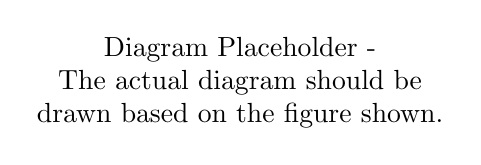
\begin{tikzpicture}
        % The diagram provided in the question was a conceptual one,
        % not suitable for replication with tikz without additional details.
        % Therefore, only a placeholder is included.
        \node at (0,0) [align=center] {Diagram Placeholder -\\ The actual diagram should be\\ drawn based on the figure shown.};
    \end{tikzpicture}
\end{center} 

\item In the graphs below, the resistance \(R\) of a superconductor is shown as a function of its temperature \(T\) for two different magnetic fields \(B_1\) (solid line) and \(B_2\) (dashed line). If \(B_2\) is larger than \(B_1\), which of the following graphs shows the correct variation of \(R\) with \(T\) in these fields?
    \begin{tasks}(2)
        \task Graph A
        \task Graph B
        \task Graph C
        \task Graph D
    \end{tasks}

\item A superconductor has \( T_c (0) = 100 K\). When a magnetic field of \(7.5\) Tesla is applied, its \(T_c\) decreases to \(75 K\). For this material one can definitely say that when
    \begin{tasks}(2)
        \task \(B = 5\) Tesla, \( T_c (B) = 80 K\)
        \task \(B = 5\) Tesla, \(75 K < T_c (B) < 100 K\)
        \task \(B = 10\) Tesla, \(75 K < T_c (B) < 100 K\)
        \task \(B = 10\) Tesla, \(T_c (B) = 70 K\)
    \end{tasks} 

    
    \item A horizontal circular platform of radius 0.5 m and mass 0.45 kg is free to rotate about its axis. Two massless spring toy-guns, each carrying a steel ball of mass 0.05 kg are attached to the platform at a distance 0.25 m from the centre on its either sides along its diameter (see figure). Each gun simultaneously fires the balls horizontally and perpendicular to the diameter in opposite directions. After leaving the platform, the balls have horizontal speed of 9 m\textsuperscript{-1} with respect to the ground. The rotational speed of the platform in\textsuperscript{-1} after the balls leave the platform is \underline{\hspace{2.5 cm}}.

    \begin{center}
        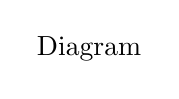
\begin{tikzpicture}
            \node {Diagram};
        \end{tikzpicture}
    \end{center}

    %  \item A circular disk of radius \(R\) carries surface charge density \(\sigma(r) = \sigma_0 \left(1 - \frac{r}{R}\right)\), where \(\sigma_0\) is a constant and \(r\) is the distance from the center of the disk. Electric flux through a large spherical surface that encloses the charged disk completely is \(\Phi_0\). Electric flux through another spherical surface of radius \(R-\frac{r}{4}\) and concentric with the disk is \(\Phi\). Then the ratio \(\frac{\Phi}{\Phi_0}\) is \underline{\hspace{2.5 cm}}.

 \begin{solution}
    \begin{align*}
        \intertext{Total charge on the disk, \(Q\), is obtained by integrating the surface charge density over the area of the disk,}
        Q &= \int_0^{2\pi} \int_0^R \sigma(r) r \, dr \, d\theta \\
        &= \int_0^{2\pi} \int_0^R \sigma_0 \left(1 - \frac{r}{R}\right) r \, dr \, d\theta \\
        &= \sigma_0 \int_0^{2\pi} \left(\int_0^R r - \frac{r^2}{R} \, dr\right) d\theta \\
        &= \sigma_0 \int_0^{2\pi} \left(\frac{R^2}{2} - \frac{R^3}{3R}\right) d\theta \\
        &= \sigma_0 (2\pi) \left(\frac{R^2}{2} - \frac{R^2}{3}\right) \\
        &= \sigma_0 (2\pi) \frac{R^2}{6} \\
        &= \frac{\sigma_0 \pi R^2}{3}
        \intertext{The electric flux \(\Phi_0\) through a large spherical surface enclosing the disk is given by,}
        \Phi_0 &= \frac{Q}{\varepsilon_0} \\
        &= \frac{\sigma_0 \pi R^2}{3\varepsilon_0}
        \intertext{The electric flux \(\Phi\) through a spherical surface of radius \(R-\frac{r}{4}\) is given by,}
        \Phi &= \frac{Q'}{\varepsilon_0}
        \intertext{where \(Q'\) is the charge inside the sphere of radius \(R-\frac{r}{4}\). Since the sphere is concentric with the disk, we need to find charge within radius \(R-\frac{r}{4}\),}
        Q' &= \int_0^{2\pi} \int_0^{R-\frac{r}{4}} \sigma(r) r \, dr \, d\theta \\
        &= \sigma_0 \int_0^{2\pi} \left(\int_0^{R-\frac{r}{4}} r - \frac{r^2}{R} \, dr\right) d\theta \\
        &= \sigma_0 \int_0^{2\pi} \left(\frac{(R-\frac{r}{4})^2}{2} - \frac{(R-\frac{r}{4})^3}{3R}\right) d\theta \\
        &= \sigma_0 (2\pi) \frac{(R-\frac{r}{4})^2}{6} \\
        &= \frac{\sigma_0 \pi (R-\frac{r}{4})^2}{3}
        \intertext{So, the ratio \(\frac{\Phi}{\Phi_0}\) is,}
        \frac{\Phi}{\Phi_0} &= \frac{\frac{\sigma_0 \pi (R-\frac{r}{4})^2}{3\varepsilon_0}}{\frac{\sigma_0 \pi R^2}{3\varepsilon_0}} \\
        &= \frac{(R-\frac{r}{4})^2}{R^2} \\
        &= \frac{R^2 - \frac{rR}{2} + \frac{r^2}{16}}{R^2} \\
        &= 1 - \frac{r}{2R} + \frac{r^2}{16R^2}
        \intertext{This is the required ratio of the electric fluxes.}
    \end{align*}
\end{solution}
    % 
    \item A horizontal circular platform of radius 0.5 m and mass 0.45 kg is free to rotate about its axis. Two massless spring toy-guns, each carrying a steel ball of mass 0.05 kg are attached to the platform at a distance 0.25 m from the centre on its either sides along its diameter (see figure). Each gun simultaneously fires the balls horizontally and perpendicular to the diameter in opposite directions. After leaving the platform, the balls have horizontal speed of 9 m\textsuperscript{-1} with respect to the ground. The rotational speed of the platform in\textsuperscript{-1} after the balls leave the platform is \underline{\hspace{2.5 cm}}.

    \begin{center}
        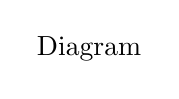
\begin{tikzpicture}
            \node {Diagram};
        \end{tikzpicture}
    \end{center}

    \item A particle of unit mass is moving along the x-axis under the influence of a force and its total energy is conserved. Four possible forms of the potential energy of the particle are given in Column I($a$ and $U_0$ are constants). Match the potential energy functions in Column I with the corresponding statement(s) in Column II.
\begin{center}
    \renewcommand{\arraystretch}{3}
    \begin{table}[h]
        \centering
        \begin{tabular}{p{0.25cm}p{5cm}|p{0.25cm}p{8cm}}
        \hline
        & Column I & & Column II \\
        \hline
        (A) & \( U_1(x) = \frac{U_0}{2} \left[ 1 - \left( \frac{x}{a} \right)^2 \right]^2 \) & (P) & The force acting on the particle is zero at \( x = a \). \\
        (B) & \( U_2(x) = \frac{U_0}{2} \left( \frac{x}{a} \right)^2 \) & (Q) & The force acting on the particle is zero at \( x = 0 \). \\
        (C) & \( U_3(x) = \frac{U_0}{2} \left( \frac{x}{a} \right)^2 \exp \left[ - \left( \frac{x}{a} \right)^2 \right] \) & (R) & The force acting on the particle is zero at \( x = -a \). \\
        (D) & \( U_4(x) = \frac{U_0}{2} \left[ \frac{x}{a} - \frac{1}{3} \left( \frac{x}{a} \right)^3 \right] \) & (S) & The particle experiences an attractive force towards \( x = 0 \) in the region \( |x| < a \). \\
         &  & (T) & The particle with total energy \( \frac{U_0}{4} \) can oscillate about the point \( x = -a \). \\
        \hline
        \end{tabular}
    \end{table}
\end{center}
\begin{solution}
    \begin{align*}
        \intertext{The force acting on the particle can be found by taking the negative derivative of the potential energy function with respect to $x$.}
        \intertext{For option (A):}
        F_1(x) &= -\dfrac{dU_1}{dx} = -\dfrac{d}{dx} \left[ \dfrac{U_0}{2} \left(1-\dfrac{x^2}{a^2}\right)^2 \right]\\
        &= -U_0 \left(\dfrac{x}{a^2}\right) \left(1-\dfrac{x^2}{a^2}\right)\\
        \intertext{The force acting on the particle is zero at \(x=0\) and \(x=\pm a\) which corresponds to option (Q) and (P)(R).}
        \intertext{For option (B):}
        F_2(x) &= -\dfrac{dU_2}{dx} = -\dfrac{d}{dx} \left[ \dfrac{U_0}{2} \left(\dfrac{x}{a}\right)^2 \right]\\
        &= -U_0 \left(\dfrac{x}{a^2}\right)\\
        \intertext{The force acting on the particle is zero at \(x=0\) which corresponds to option (Q).}
        \intertext{For option (C):}
        F_3(x) &= -\dfrac{dU_3}{dx} = -\dfrac{d}{dx} \left[ \dfrac{U_0}{2} \left(\dfrac{x}{a}\right)^2 \exp\left(-\dfrac{x^2}{a^2}\right) \right]\\
        &= -U_0 \left(\dfrac{x}{a^2}\right) \exp\left(-\dfrac{x^2}{a^2}\right) \left(1 - 2\dfrac{x^2}{a^2}\right)\\
        \intertext{The force acting on the particle is zero at \(x=0\) and \(x=\pm a/\sqrt{2}\) which corresponds to option (Q).}
        \intertext{For option (D):}
        F_4(x) &= -\dfrac{dU_4}{dx} = -\dfrac{d}{dx} \left[ \dfrac{U_0}{2} \left(\dfrac{x}{a} - \dfrac{1}{3}\left(\dfrac{x}{a}\right)^3 \right) \right]\\
        &= U_0 \left(\dfrac{1}{a} - \dfrac{x^2}{a^3}\right)\\
        \intertext{The force acting on the particle is zero at \(x=\pm a\) which corresponds to option (P) and (R). Also, in the region \(|x|<a\) the term inside the parentheses is positive, so the force acting on the particle is towards \(x=0\) which corresponds to option (S).}
    \end{align*}
\end{solution}
    \item What is the minimum acceleration with which bar \( A \) (Fig. 1.22) should be shifted horizontally to keep bodies \( 1 \) and \( 2 \) stationary relative to the bar? The masses of the bodies are equal, and the coefficient of friction between the bar and the bodies is equal to \( k \). The masses of the pulley and the threads are negligible, the friction in the pulley is absent.
    \begin{center}
        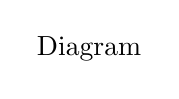
\begin{tikzpicture}
            \node at (0, 0) {Diagram};
        \end{tikzpicture}
    \end{center}
    \item Prism 1 with bar 2 of mass \( m \) placed on it gets a horizontal acceleration \( w \) directed to the left (Fig. 1.23). At what maximum value of this acceleration will the bar be still stationary relative to the prism, if the coefficient of friction between them \( k < \cot \alpha \)?
    \begin{center}
        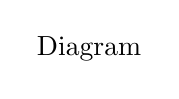
\begin{tikzpicture}
            \node at (0, 0) {Diagram};
        \end{tikzpicture}
    \end{center}
    \item Prism 1 of mass \(m_1\) and with angle \(\alpha\) (see Fig. 1.23) rests on a horizontal surface. Bar 2 of mass \(m_2\) is placed on the prism. Assuming the friction to be negligible, find the acceleration of the prism. 
    \begin{center}
        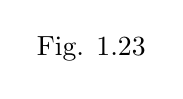
\begin{tikzpicture}
            \node at (0, 0) {Fig. 1.23};
        \end{tikzpicture}
    \end{center}\begin{solution}
    \begin{center}
        \begin{tikzpicture}
            \pic at (0, 0) {frame=3cm};
        \end{tikzpicture}
    \end{center}
    
    \begin{align*}
        \intertext{Let us draw the force diagram of each body, and on this basis we observe that the prism moves towards right (say) with an acceleration $\vec{w}_1$ and the bar 2 of mass $m_2$ moves down the plane with respect to 1, say with acceleration $\vec{w}_{21}$, then}
        \vec{w}_2 &= \vec{w}_{21} + \vec{w}_1 \quad \text{(see figure).}
        \intertext{Let us write Newton’s second law of both bodies in projection form along positive $y_2$ and $x_1$ axes as shown in the figure.}
        m_2 g \cos \alpha - N &= m_2 w_{2(y_2)} = m_2 [w_{21(y_2)} + w_{1(y_2)}] = m_2 [0 + w_1 \sin \alpha]
        \intertext{or}
        m_2 g \cos \alpha - N &= m_2 w_1 \sin \alpha \tag{1}
        \intertext{and}
        N \sin \alpha &= m_1 w_1 \tag{2}
        \intertext{Solving Eqs. (1) and (2), we get}
        w_1 &= \dfrac{m_2 g \sin \alpha \cos \alpha}{m_1 + m_2 \sin^2 \alpha} = \dfrac{g \sin \alpha \cos \alpha}{(m_1/m_2) + \sin^2 \alpha}
    \end{align*}
\end{solution}
    
\item A radius vector of a point A relative to the origin varies with time \( t \) as \( \mathbf{r} = at\mathbf{i} - bt^3\mathbf{j} \), where \( a \) and \( b \) are positive constants, and \( \mathbf{i} \) and \( \mathbf{j} \) are the unit vectors of the \( x \) and \( y \) axes. Find:
    \begin{enumerate}
        \item the equation of the point's trajectory \( y(x) \); plot this function;
        \item the time dependence of the velocity \( \mathbf{v} \) and acceleration \( \mathbf{w} \) vectors, as well as of the moduli of these quantities;
        \item the time dependence of the angle \( \alpha \) between the vectors \( \mathbf{w} \) and \( \mathbf{v} \);
        \item the mean velocity vector averaged over the first \( t \) seconds of motion, and the modulus of this vector.
    \end{enumerate}

\begin{solution}
    \begin{center}
        \begin{tikzpicture}
            \pic at (0, 0) {frame=3cm};
        \end{tikzpicture}
    \end{center}
    
    \begin{align*}
        \intertext{(a) As}
        \vec{r} &= at\hat{i} - bt^2\hat{j} \\
        \intertext{So,}
        x &= at,\ y = -bt^2 \\
        \intertext{and therefore}
        y &= \dfrac{-bx^2}{a^2}
        \intertext{which is equation of a parabola, whose graph is shown in the figure.}
        \intertext{(b) As}
        \vec{r} &= at\hat{i} - bt^2\hat{j} \\
        \intertext{So,}
        \vec{v} &= \dfrac{d\vec{r}}{dt} = a\hat{i} - 2bt\hat{j} \tag{1} \\
        v &= \sqrt{a^2 + (-2bt)^2} = \sqrt{a^2 + 4b^2t^2}
        \intertext{Differentiating Eq. (1) with respect to time, we get}
        \vec{w} &= \dfrac{d\vec{v}}{dt} = -2b\hat{j} \\
        \intertext{So,}
        |\vec{w}| &= w = 2b \\
        \intertext{(c)}
        \cos{\alpha} &= \dfrac{\vec{v} \cdot \vec{w}}{vw} = \dfrac{(a\hat{i} - 2bt\hat{j}) \cdot (-2b\hat{j})}{(\sqrt{a^2 + 4b^2 t^2}) 2b} \\
        \intertext{or}
        \cos{\alpha} &= \dfrac{2bt}{\sqrt{a^2 + 4b^2 t^2}} \\
        \intertext{So,}
        \tan{\alpha} &= \dfrac{a}{2bt}\ \text{or}\ \alpha = \tan^{-1}\left(\dfrac{a}{2bt}\right)
        \intertext{(d) The mean velocity vector}
        \left<\vec{v}\right> &= \dfrac{\int{\vec{v} dt}}{\int dt} = \dfrac{\int_0^t (a\hat{i} - 2bt\hat{j}) dt}{t} = a\hat{i} - bt\hat{j} \\
        \intertext{Hence,}
        \left<|\vec{v}|\right> &= \sqrt{a^2 + (-bt)^2} = \sqrt{a^2 + b^2 t^2}
    \end{align*}
\end{solution}

    \item A smooth light horizontal rod \(AB\) can rotate about a vertical axis passing through its end \(A\). The rod is fitted with a small sleeve of mass \(m\) attached to the end \(A\) by a weightless spring of length \(l_0\) and stiffness \(\kappa\). What work must be performed to slowly get this system going and reaching the angular velocity \(\omega\)?
\begin{solution}
    \begin{center}
        \begin{tikzpicture}
            \pic at (0, 0) {frame=3cm};
        \end{tikzpicture}
    \end{center}
    
    \begin{align*}
        \intertext{Let the deformation in the spring be $\Delta l$, when the rod $AB$ has attained the angular velocity $\omega$. From the second law of motion in projection form $F_n = mwv_n$.}
        \kappa \Delta l &= m \omega^2 \left(l_0 + \Delta l \right)  \quad \text{or} \quad \Delta l = \dfrac{m\omega^2 l_0}{\kappa - m \omega^2}
        \intertext{From the energy equation, $A_{ext}$}
        A_{ext} &= \dfrac{1}{2} mv^2 + \dfrac{1}{2} \kappa \Delta l^2\\
        &= \dfrac{1}{2} m \omega^2 \left(l_0 + \Delta l\right)^2 + \dfrac{1}{2} \kappa \Delta l^2\\
        &= \dfrac{1}{2} m \omega^2 \left( l_0 + \dfrac{m \omega^2 l_0}{\kappa - m \omega^2}\right)^2 + \dfrac{1}{2} \kappa \left(\dfrac{m \omega^2 l_0}{\kappa - m \omega^2}\right)^2
        \intertext{On solving}
        A_{ext} &= \dfrac{\kappa l_0^2 \eta \left(1 + \eta\right)}{2 \left(1 - \eta\right)^2}, \quad \text{where} \quad \eta = \dfrac{m \omega^2}{\kappa}
    \end{align*}
\end{solution}

    
\item A point moves in the plane $xy$ according to the law $x = a \sin \omega t$, $y = a(1 - \cos \omega t)$, where $a$ and $\omega$ are positive constants. Find:
    \begin{enumerate}
        \item the distance $s$ traversed by the point during the time $t$;
        \item the angle between the point's velocity and acceleration vectors.
    \end{enumerate}

    \item Two interacting particles form a closed system whose centre of inertia is at rest. Fig. 1.36 illustrates the positions of both particles at a certain moment and the trajectory of the particle of mass $m_1$. Draw the trajectory of the particle of mass $m_2$ if $m_2 = m_1/2$.
    \begin{center}
        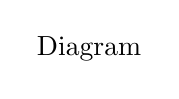
\begin{tikzpicture}
            \node at (0, 0) {Diagram};
        \end{tikzpicture}
    \end{center}\begin{solution}
    \begin{center}
        \begin{tikzpicture}
            \pic at (0, 0) {frame=3cm};
        \end{tikzpicture}
    \end{center}
    
    \begin{align*}
        \intertext{As the closed system consisting of two particles $m_1$ and $m_2$ is initially at rest, the centre of mass of the system will remain at rest. Further as $m_2 = m_1/2$, the centre of mass of the system divides the line joining $m_1$ and $m_2$ at all the moments of time in the ratio 1:2. In addition to it, the total linear momentum of the system at all the times is zero.}
        \vec{p}_1 &= -\vec{p}_2 
        \intertext{and therefore the velocities of $m_1$ and $m_2$ are also directed in opposite sense. Bearing in mind all these things, the sought trajectory is as shown in the figure.}
    \end{align*}
\end{solution}
    \item An LCR series circuit of capacitance 62.5nF and resistance of 50$\Omega$, is connected to an A.C. source of frequency 2.0 kHz. For maximum value of amplitude of current in circuit, the value of inductance is \underline{\hspace{4cm}} mH. (Take $\pi^2 = 10$)
\end{enumerate}
\end{document}